% Document definitions
\documentclass{article}
\usepackage[right=8mm, left=8mm, top=5mm, bottom=7mm, landscape]{geometry}
\usepackage[utf8]{inputenc}
\usepackage{multicol}
\usepackage{graphicx}
\usepackage[yyyymmdd]{datetime}
\usepackage{url}
\usepackage{hyperref}
\usepackage{multirow}
\usepackage{enumitem}

% Fonts and colors
\usepackage{CJKutf8}
\usepackage{xcolor}
\usepackage{sectsty}
\setlength{\columnsep}{8mm}
\definecolor{headings}{HTML}{3E0E82}
\chapterfont{\color{headings}}
\sectionfont{\color{headings}}
\subsectionfont{\color{headings}}
\subsubsectionfont{\color{headings}}
\hypersetup{pdfstartview=FitH, colorlinks, linkcolor={blue}, citecolor={blue}, urlcolor={blue}}
\newlist{colorize}{itemize}{1}
\setlist[colorize]{label=\textcolor{headings}{\textbullet},itemsep=1pt,topsep=2pt}
\setlist[enumerate]{label=\color{headings}\textbf{\theenumi.},itemsep=1pt,topsep=2pt}

% Document
\begin{document}
\begin{CJK}{UTF8}{min}

\begin{center}
{\color{headings}\scshape\large{Japanese Language Reference - Ver. \today}}
\end{center}

\begin{multicols*}{3}

\section{Introduction to Japanese}

This document is the result of my notes and reference guide while learning the language. I provide it here for free under the 
\href{https://creativecommons.org/licenses/by-sa/4.0/}{\texttt{CC BY-SA}} license. You can find the latest version at \url{http://dendory.net}. If you find any mistake or want to 
send your comments, feel free to contact me at \href{mailto:dendory@live.ca}{\texttt{dendory@live.ca}}. Copyright 2018 Patrick Lambert.

\subsection{Alphabets}

The Japanese language uses 3 different alphabets:

\begin{colorize}
\item Hiragana
\item Katakana
\item Kanji
\end{colorize}

Hiragana has 46 characters and is similar to the English alphabet. It's used to construct sentences, along with connecting words. Katakana follows the same pattern and is used for 
English origin words, along with words that you want to put emphasis on. Both are phonetic alphabets. Kanji are characters which come from the Chinese alphabet and are used for words of 
Chinese origin. There are over 10,000 kanjis but you only need to learn about 2,000 for fluency.

\subsubsection{Hiragana}
\begin{tabular}{|c|c|c|c|c|}
%\hline
%\multicolumn{5}{ |c| }{Hiragana} \\
\hline
あ&い&う&え&お\\
a&i&u&e&o\\ \hline
か&き&く&け&こ\\
ka&ki&ku&ke&ko\\ \hline
が&ぎ&ぐ&げ&ご\\
ga&gi&gu&ge&go\\ \hline
さ&し&す&せ&そ\\
sa&shi&su&se&so\\ \hline
ざ&じ&ず&ぜ&ぞ\\
za&ji&zu&ze&zo\\ \hline
た&ち&つ&て&と\\
ta&chi&tsu&te&to\\ \hline
だ&ぢ&づ&で&ど\\
da&ji&zu&de&do\\ \hline
な&に&ぬ&ね&の\\
na&ni&nu&ne&no\\ \hline
\end{tabular}
\begin{tabular}{|c|c|c|c|c|}
\hline
は&ひ&ふ&へ&ほ\\
ha&hi&fu&he&ho\\ \hline
ば&び&ぶ&べ&ぼ\\
ba&bi&bu&be&bo\\ \hline
ぱ&ぴ&ぷ&ぺ&ぽ\\
pa&pi&pu&pe&po\\ \hline
ま&み&む&め&も\\
ma&mi&mu&me&mo\\ \hline
ら&り&る&れ&ろ\\
ra&ri&ru&re&ro\\ \hline
や&&ゆ&&よ\\
ya&&yu&&yo\\ \hline
わ&&&&を\\
wa&&&&wo\\ \hline
&&&&ん\\
&&&&n\\ \hline
\end{tabular}

On top of the regular symbols, you can also make additional sounds with a smaller version of certain symbols. For example, きよ is \textit{kiyo} while きょ is \textit{kyo}. The っ 
symbol can also be used to double a consonant. For example, やっぱり (as I thought) is spelled \textit{yappari}. Another important phonetic note is that the \textit{u} vowel is often 
omitted. For example, です (is) can be spoken as \textit{desu} or \textit{des}, while こうこう (high school) can be written \textit{koukou} but sounds like \textit{koko}.

\subsubsection{Katakana}
\begin{tabular}{|c|c|c|c|c|}
\hline
ア&イ&ウ&エ&オ\\
a&i&u&e&o\\ \hline
カ&キ&ク&ケ&コ\\
ka&ki&ku&ke&ko\\ \hline
ガ&ギ&グ&ゲ&ゴ\\
ga&gi&gu&ge&go\\ \hline
サ&シ&ス&セ&ソ\\
sa&shi&su&se&so\\ \hline
ザ&ジ&ズ&ゼ&ゾ\\
za&ji&zu&ze&zo\\ \hline
タ&チ&ツ&テ&ト\\
ta&chi&tsu&te&to\\ \hline
ダ&ヂ&ヅ&デ&ド\\
da&ji&zu&de&do\\ \hline
ナ&ニ&ヌ&ネ&ノ\\
na&ni&nu&ne&no\\ \hline
\end{tabular}
\begin{tabular}{|c|c|c|c|c|}
\hline
ハ&ヒ&フ&ヘ&ホ\\
ha&hi&fu&he&ho\\ \hline
バ&ビ&ブ&ベ&ボ\\
ba&bi&bu&be&bo\\ \hline
パ&ピ&プ&ペ&ポ\\
pa&pi&pu&pe&po\\ \hline
マ&ミ&ム&メ&モ\\
ma&mi&mu&me&mo\\ \hline
ラ&リ&ル&レ&ロ\\
ra&ri&ru&re&ro\\ \hline
ヤ&&ユ&&ヨ\\
ya&&yu&&yo\\ \hline
ワ&&&&ヲ\\
wa&&&&wo\\ \hline
&&&&ン\\
&&&&n\\ \hline
\end{tabular}

The sounds are just like the Hiragana version, only with different symbols. On top of the notes above, the ー symbol can be used to double a vowel. For example, ケーキ (cake) sounds 
like \textit{keeki}.

\subsubsection{Kanji}

There are many kanjis and they all have several sounds. Some are simple like 日 (day, sun) or 木 (tree). Some are made up of several simpler kanjis like 森 (forest) being composed of 
3 trees. Some look like objects like 車 (car) which looks like two wheels on the side of a vehicle, while others don't really look like much of anything, such as 雲 (cloud).

The way they sound depends on whether the kanji is paired with other kanjis, such as 日本 (Japan) being spelled as にほん, or whether they are paired with hiragana or katakana 
characters, such as この日 (this day) which is spelled このひ. A single kanji can have many spellings, and only context determines which spelling to use. It's also possible to 
determine what a compound word means based on its components, such as 休日 [くうじつ] (holiday) being composed of 休 (rest) and 日 (day).

\subsection{Numbers}

The basic number system in Japanese employs the following digits:

\begin{colorize}
\item 〇 [れい] - zero
\item 一 [いち] - one
\item 二 [に] - two
\item 三 [さん] - three
\item 四 [し, よん] - four
\item 五 [ご] - five
\item 六 [ろく] - six
\item 七 [しち, なな] - seven
\item 八 [はち] - eight
\item 九 [く, きゅう] - nine
\item 十 [じゅ] - ten
\item 百 [ひゃく] - hundred
\item 千 [せん] - thousand
\item 万 [いちまん] - ten thousand
\end{colorize}

To create any number, you can use a combination of these symbols. For example, the number 73 is 七十三 [しちじゅさん] while the number 21,318 is 二万千三百十八 
[にせんさんひゃくじゅはち]. Note that some numbers are spoken in a slightly different way, such as 300 is 三百 is spelled さんびゃく instead of さんひゃく. Another important thing to 
note is that Japanese uses counters. This typically starts with the number, followed by another symbol, depending on what you're trying to count. For example, counting people you 
would add 人 [じん] to give you: 一人 [ひとり] (one person), 二人 [ふたり] (two people), 三人 [さんにん] (three people), 四人 [よにん] (four people). In this case, one person and two 
people have their own spellings, but after that you just add 。。。にん. For objects, the counter is つ which gives you: 一つ [ひとつ] (one object), 二つ [ふたつ] (two objects), 三つ 
[みっつ] (three objects), 四つ [よっつ] (four objects) and so on.

\subsection{Sentence composition}

To create sentences once you know the alphabets, you also need to know about a few basic components of the Japanese language. These include the politeness level and honorifics, 
particles, copula and word order.

\subsubsection{Honorifics and politeness}

Japanese people are a very polite species, and as such the language has several levels of politeness. Depending on who you ask, there can be up to 4 or 5 levels, although usually 
it's enough to understand the difference between casual and polite speak. Typically, speaking casually will be quicker, words will be shorter, and many words can be omitted. Slang is 
also considered casual, and honorifics will change as well.

When talking to someone or about somebody, the あなた (you) word is rarely used. Instead, you're expected to use the person's name or title with the proper honorific. Here are the 
most common ones:

\begin{colorize}
\item 。。。さん - Common honorific for people of your status.
\item 。。。さま - Very polite, used for elders or God.
\item 。。。くん - Casual, used for guys.
\item 。。。ちゃん - Casual, used for girls.
\item 。。。たん - Casual, used for little kids.
\end{colorize}

Always use the name or title, followed by the proper honorific. For example, when talking to a girl named Sakura in a casual way, you can say さくらちゃん. When talking to a stranger 
named Hiroshi, you would use ひろしさん. You can also switch them based on how polite you want to be, like おねえさん (older sister, polite) and おねえちゃん (older sister, casual).

On top of different honorifics and sentence composition, words (especially verbs) will also change based on whether you're being casual or polite. For example, 食べる (eat) is 
the casual version, while 食べます (eat) is the polite version, also called the \textit{masu form}. Here is the verb conjugated both ways:
\begin{tabular}{@{}|l|l|l|l|@{}}
\hline
\multicolumn{4}{ |c| }{\textbf{食べる [たべる] (to eat)}} \\
\hline
I eat
&I don't eat
&I ate
&Eat!
\\\hline
食べる
&食べない
&食べた
&食べて
\\
食べます
&食べません
&食べました
&
\\ \hline
\end{tabular}

Verbs have a past and non-past tense. There is no future tense, instead the context is used.

Finally, you will see the suffixes なさい and ございます added to certain words. For example, おはよう (good morning) can be made more polite by saying おはようございます.

\subsubsection{Particles}

In English, the word order is always fixed. Also, we use spaces in order to clearly separate words. In Japanese, word order is flexible, and there are no spaces in Japanese books. 
This means words have to be identified by particles in order to see the context. These are the most used particles:

\begin{colorize}
\item は (spelled 'wa') - Topic marker, follows the subject of the sentence.
\item を (spelled 'o') - Object marker, follows the object of the sentence.
\item が - Object marker for action verbs.
\item に - Location marker, follows a static location where something is.
\item で - Location marker, follows a location where an action occurs.
\item の - Possessive marker, basically the same as \textit{'s}.
\end{colorize}

For example, if you have the name Sakura and the sentence has this person being the subject, the は particle would follow. Similarly, if 私 [わたし] (I, myself) is in the sentence, 
but the subject is an object I own, you would use the の particle. Two additional particles of interest that can usually only be found at the end of sentences are ね (isn't it?) and 
よ (yo) which are ways to be more expressive. For example, そうですね (it is so, isn't it?).

\subsubsection{Word order}

The word order in English is SVO (subject verb object). However in Japanese it's SOV (subject object verb). So when you would normally say \textit{Sakura eats cake}, the Japanese 
version would be さくらはケーキを食べます (Sakura cake eats). The sentence can be divided in the following parts:

\begin{colorize}
\item さくら - Topic
\item は - Topic marker
\item ケーキ - Object
\item を - Object marker
\item 食べます - Verb
\end{colorize}

\subsubsection{Copula}

A copula is a way to link subjects to predicates. Basically, the word でございます (is) which is used to end sentences when the verb of the sentence is \textit{to be}. In common usage, 
it's shortened to です for polite conversations, and だ for casual ones. For example: 私は日本人です (I am Japanese) contains the subject 私 [わたし] (I), the は topic marker, the 
object 日本人 [にほんじん] (Japanese) and the copela です (is).

Note that the subject is often dropped when it's obvious from the context. So in this case you would just say 日本人です. It's also commonly used when talking about yourself. For 
example, if someone asks お元気[げんき]ですか (how are you?) you can answer 元気です (I am feeling well). Similarly, when introducing yourself you should say your name followed by 
です. In a casual setting, you can use だ instead, or skip the copela completely.

\subsubsection{Common expressions}

There are a lot of common expressions that you will hear countless times in a typical conversation without any real relation with the topic of discussion. These are ways to agree 
with someone, think additional points of conversation, or exclaim excitement. Here are some of the most common expressions:

\begin{colorize}
\item そうですね - It is, isn't it?
\item そうですか - I guess it is.
\item やっぱり - I knew it!
\item そっか, なるほど - I see...
\item やった - I did it!
\item あの。。。 - Uhm...
\item よかった - That was good!
\item いいですね, いいから - That's good.
\item ちょっと待[ま]って - Wait a moment!
\item どうぞ - Go ahead.
\item かしら, かな - I wonder.
\item いただきます - Let's eat!
\item しょがない - It can't be helped.
\item 大丈夫 [だいじょうぶ] - I'm alright.
\item こちらこそ - Same here, likewise
\item だめよ - It's no good!
\item がんばって - Good luck!
\end{colorize}

The word いい (good) is an adjective used in a lot of sentences to describe something that is OK or good. そう (so) means the same in English, while 大丈 [だいじょうぶ] (I'm alright) 
starts with the word 大 [おお] (big), used in many sentences to imply a strong sense of something. For example, 好[す]きです (I like you) versus 大[だい]好[す]きです (I love 
you).

こちら means \textit{over here}, while ちょっと in ちょっと待って means \textit{a little bit}.
\begin{tabular}{@{}|l|l|l|l|@{}}
\hline
\multicolumn{4}{ |c| }{\textbf{待つ [まつ] (to wait)}} \\
\hline
I wait
&I don't wait
&I waited
&Wait!
\\\hline
待つ
&待たない
&待った
&待って
\\
待ちます
&待ちません
&待ちました
&
\\ \hline
\end{tabular}

\subsubsection{Pronouns}

The words \textit{I} and \textit{you} aren't used much in Japanese for two reasons. First, the subject is often omitted when the context makes it clear. Also, you're expected to use 
the person's name when you know it, even if you're talking directly to them. Still, there are several pronouns that can be useful to know in certain situations:

\begin{colorize}
\item 私 [わたし] - I, myself
\item ぼく, おれ - I, myself (only guys)
\item あなた - You
\item きみ - You (casual)
\item 私達 [わたしたち] - We
\end{colorize}

For example, you can say 私達は東京に行きました [わたしたちはとうきょうにいきました] (We went to Tokyo). Since the verb doesn't change in the plural form (in this case 行く is in the 
past, polite form) then the subject is required.
\begin{tabular}{@{}|l|l|l|l|@{}}
\hline
\multicolumn{4}{ |c| }{\textbf{行く [いく] (to go)}} \\
\hline
I go
&I don't go
&I went
&Go!
\\\hline
行く
&行かない
&行った
&行って
\\
行きます
&行きません
&行きました
&
\\ \hline
\end{tabular}

\subsection{Greetings}

Greetings are among the first thing you may want to do in Japanese, and what typically begins a conversation.

\begin{colorize}
\item はじめまして - Nice to meet you.
\item お元気[げんき]ですか - How are you feeling?
\item よろしくお願[ねがい]いします - Let's do our best.
\item おはよう - Good morning.
\item こんにちは - Good day.
\item こんばんは - Good evening.
\item 行[い]って来[き]ます - I'll be back later!
\item じゃまたね - See you later!
\item ただいま - I'm back!
\item お帰[かえ]り - Welcome back!
\item おやすみ - Good night.
\end{colorize}

The expression 行って来ます (I'll be back later) uses two common verbs, to go and to come. They are often used alongside other verbs to indicate an action you're about to do.\\
\begin{tabular}{@{}|l|l|l|l|@{}}
\hline
\multicolumn{4}{ |c| }{\textbf{来る [くる] (to come)}} \\
\hline
I come
&I don't come
&I came
&Come!
\\\hline
来る
&来ない
&来た
&来て
\\
来ます
&来ません
&来ました
&
\\ \hline
\end{tabular}

\subsection{Asking questions}

Any sentence can be changed into a question by adding か at the end. For example, あなたはアメリカ人です (You are American) can be changed to a question with あなたはアメリカ人ですか 
(Are you American?). Note that アメリカ is in katakana since it's a foreign word.

While adding か at the end of a sentence will automatically make it into a question, there are specific words that you need to know in order to ask some of the most basic questions 
from other people. Here are the most common ones:

\begin{colorize}
\item 何 [なに, なん] - What?
\item どこ - Where?
\item どう - How?
\item 誰 [だれ] - Who?
\item どれ - Which?
\item いつ - When?
\item 何で, なぜ, どうして - Why?
\item いくら - How much?
\end{colorize}

The most common of these is 何 [ なん] (what) which can be paired with other words to ask questions. For example, 歳 [さい] (years old) can be used to ask someone's age like this: 
何歳ですか. The word 時 [じ] (o'clock) can be used to ask the time like this: 何時ですか. To ask someone to repeat an answer, say もう一度 [もういちど] (once more).

When talking about doing something, the verb する (to do) comes up often, usually paired with other verbs. It can also be used in simple sentences like: 私はします (I will do it).
\begin{tabular}{@{}|l|l|l|l|@{}}
\hline
\multicolumn{4}{ |c| }{\textbf{する (to do)}} \\
\hline
I do
&I don't do
&I did
&Do!
\\\hline
する 
&しない
&した
&して
\\
します
&しません
&しました
&
\\ \hline
\end{tabular}

For simple questions, you may be able to answer with はい (yes) or いいえ (no). For more complex ones, you may need the verb \textit{to be} to say that someone or something is in 
some state, or that something exists. This is actually divided in two verbs in Japanese: いる is for living beings (humans, pets) while ある is for objects. It's not rare to use 
あります (is) or ありません (is not) as positive and negative affirmations.
\begin{tabular}{@{}|l|l|l|l|@{}}
\hline
\multicolumn{4}{ |c| }{\textbf{ある (to be)}} \\
\hline
It is
&It's not
&It was
&Be!
\\\hline
ある
&ない
&あった
&あって
\\
あります
&ありません
&ありました
&
\\ \hline
\end{tabular}
\begin{tabular}{@{}|l|l|l|l|@{}}
\hline
\multicolumn{4}{ |c| }{\textbf{いる (to be)}} \\
\hline
I am
&I am not
&I was
&Be!
\\\hline
いる
&いない
&いた
&いて
\\
います
&いません
&いました
&
\\ \hline
\end{tabular}

\clearpage

\section{Basic concepts}

After covering the basics of constructing words and sentences, there are still plenty more basic abstract concepts such as telling time and referring to groups of people.

\subsection{Time and dates}

時 [とき] (time) can be told using 時間 [じかん] (hours) and 分間 [ぶんかん] (minutes). To say a specifc time during the day, you would use the number of hours, followed with 時 [じ] 
(o'clock), and then the number of minutes with 分 [ぶん, ふん]. For example, 3:17 would be 三時十七分. To say \textit{and a half} you can use 半 [はん]. So 2:30 would be 二時半. You can 
also add seconds with 秒 [びょう]. The act of looking at a clock would be 時計を見る [とけいをみる].
\begin{tabular}{@{}|l|l|l|l|@{}}
\hline
\multicolumn{4}{ |c| }{\textbf{見る [みる] (to look)}} \\
\hline
I look
&I don't look
&I looked
&Look!
\\\hline
見る
&見ない
&見た
&見て
\\
見ます
&見ません
&見ました
&
\\ \hline
\end{tabular}

For dates, here are the important words to know:

\begin{colorize}
\item 日 [ひ, にち] - Day
\item 週 [しゅう] - Week
\item 月 [つき, がつ, げつ] - Month
\item 年 [とし, ねん] - Year
\end{colorize}

So to tell a specific date you would use: 2019年6月15日 [二千十九ねん六がつ十五にち].

\subsubsection{Days of the week}

These are Monday through Friday, along with the work week and weekend:

\begin{colorize}
\item 月曜日 [げつようび] - Monday
\item 火曜日 [かようび] - Tuesday
\item 水曜日 [すいようび] - Wednesday
\item 木曜日 [もくようび] - Thursday
\item 金曜日 [きにようび] - Friday
\item 土曜日 [どようび] - Saturday
\item 日曜日 [にちようび] - Sunday
\item 週間 [しゅうかん] - Work week
\item 週末 [しゅうまつ] - Weekend
\end{colorize}

\subsubsection{Months of the year}

Months are the number 1 to 12 followed by 月 [がつ]. So January is 一月 [いちがつ], February is 二月 [にがつ], March is 三月 [さんがつ], April is 四月 [よんがつ] and December is 
一十月 [にじゅがつ]. They are also often written with numbers, such as 6月.

\subsubsection{Specific times of day}

Here are a few more useful terms for narrowing down a period of time:

\begin{colorize}
\item 今 [いま] - Right now
\item 今日 [きょう] - Today
\item 朝 [あさ] - Morning
\item 午前 [ごぜん] - AM
\item 午后 [ごご] - PM
\item 夜 [よる] - Night
\item 誕生日 [たんじょうび] - Birthday
\item 休日 [きゅうじつ] - Holiday
\end{colorize}

6 AM would be translated as 午前6時. You can ask \textit{what time is it right now?} with 今何時ですか [いまなんじですか]. To say you're \textit{looking forward} to a specific time 
or event, you would say 楽しみに [たのしみに].

\subsubsection{Relative dates}

You can use 次 [つぎ] (next) to speak about an upcoming event or time. For example, to say \textit{in the next 5 minutes} you can use 次の5分間. But when speaking about specific 
dates, you would use these specific terms:

\begin{colorize}
\item 明日 [あした] - Tomorrow
\item 昨日 [きのう] - Yesterday
\item 毎日 [まいにち] - Every day
\item 来週 [らいしゅう] - Next week
\item 先週 [せんしゅう] - Last week
\item 毎週 [まいしゅう] - Every week
\item 来月 [らいげつ] - Next month
\item 先月 [せんげつ] - Last month
\item 毎月 [まいつき] - Every month
\item 数日後 [すうじつご] - A few days later
\end{colorize}

To say a specific date in the next week, for example \textit{next Tuesday}, you would use 来週の火曜日 which literally means \textit{next week's Tuesday}. To say \textit{tomorrow's 
morning} you would use 明日の朝. You can also specify a time period with から (from) and まで (to) with the following structure: 6時から8時まで (from 6h to 8h).

\subsection{Groups}

Grouping people, objects or locations can be very useful when referring to things. There are common words and symbols used throughout this section to refer to people, places and things.

\subsubsection{This, that, that over there}

These are 3 useful words to refer to things:

\begin{colorize}
\item これ - This
\item それ - That
\item あれ - That over there
\end{colorize}

For example you can refer to an object in the sentence これを読む [これをよむ] (I read this) or それを読む [それをよむ] (I read that). To refer to a specific item, replace れ 
with の, like this: この本を読む [このほんをよむ] (I read this book). You can also use ここ to mean \textit{here}.
\begin{tabular}{@{}|l|l|l|l|@{}}
\hline
\multicolumn{4}{ |c| }{\textbf{読む [よむ] (to read)}} \\
\hline
I read
&I don't read
&I read (past)
&Read!
\\\hline
読む
&読まない
&読んだ
&読んで
\\
読みます
&読みません
&読みました
&
\\ \hline
\end{tabular}

\subsubsection{Crowds}

The following terms refer to crowds, specific people in the crowd, specific objects or specific locations:

\begin{colorize}
\item 日本人 [にほんじん] - Japanese
\item 外人 [がいじん] - Foreigner
\item 皆 [みんな] - Everyone
\item すべて - All
\item いっぱい - Lots
\item 誰か [だれか] - Someone
\item 誰でも [だれでも] - Anyone
\item 誰も [だれも] - No one
\item どこか - Somewhere
\item どこでも - Anywhere
\item どこにも - Nowhere
\item 何か [なにか] - Something
\item 何でも [なんでも] - Anything
\item 何も [なにも] - Nothing
\end{colorize}

Note that in some cases 皆 can also mean \textit{someone} as in 皆が英語を話すか [みんながえいごをはなすか] (does someone speak English?)
\begin{tabular}{@{}|l|l|l|l|@{}}
\hline
\multicolumn{4}{ |c| }{\textbf{話す [はなす] (to speak)}} \\
\hline
I speak
&I don't speak
&I spoke
&Speak!
\\\hline
話す
&話さない
&話した
&話して
\\
話します
&話しません
&話しました
&
\\ \hline
\end{tabular}

\subsubsection{Me too, also, however}

A few more sentence structures are needed when dealing with multiple people, objects or events. First, you may want to say \textit{me too} with the phrase 私も [わたしも]. This can 
also apply to other people, for example さくらさんも. To specify multiple people, you can use the と character between subjects: 私とさくらは食べる (me and Sakura eat). The same can 
be used for multiple objects: ケーキとパイが好きです (I like cake and pie). In the case of past-tense events, you would instead use とき or たら. To say \textit{something such as} 
you can use とか such as: ごはんとかケーキが好きです (I like things such as cake and rice).

In order to say \textit{but} you can use でも at the start of a sentence or けど at the end of a sentence. けど is also used when the second sentence is implied, to soften the first. 
You can also link two sentences together with しかし (however) or それでも (despite that).

If you're answering a question or commenting on a statement, you can start the sentence with 確かに [たしかに] (surely) in order to agree with the statement, or 別に[べつに] 
(separately) to disagree with the statement. For example, someone tells you 本当に可愛い! [ほんとおにかわいい!] (really cute!) but you disagree, you can say 別に! To follow a 
thought with another, use だらか (therefore) or じゃ (then).

\subsubsection{Family members}

A number of words can be used to describe family members, or family related things.

\begin{colorize}
\item 家族 [かぞく] - Family
\item 結婚 [けっこん] - Wedding
\item 夫 [おっと] - Husband
\item 妻 [つま] - Wife
\item お父さん [おとうさん, ちち] - Father
\item お母さん [おかあさん, はは] - Mother
\item お爺さん [おじいさん] - Grand father
\item お婆さん [おばあさん] - Grand mother
\item お兄さん [おにいさん] - Older brother
\item お姉さん [おねえさん] - Older sister
\item 伯叔 [はくしゅく] - Brothers
\item 姉妹 [しまい] - Sisters
\end{colorize}

Note that honorifics can also vary here. お姉さん (older sister, polite), お姉さま (older sister, very polite) and お姉ちゃん (older sister, casual) are all valid, depending on how 
close the two family members are to each other.

\subsection{Feelings and emotions}

Here are some of the most common adjectives used to convey 気持ち [きもち] (feelings) and 想い [おもい] (thoughts) in a casual conversation:

\begin{colorize}
\item 可愛い [かわいい] - Cute
\item 綺麗 [きれい] - Beautiful, clean
\item 面白い [おもしろい] - Interesting, funny
\item 楽しい [たのしい] - Fun
\item 大きい [おおきい] - Big
\item 少し [すこし] - Small
\item 嬉しい [うれしい] - Happy, glad
\item 格好いい [かっこういい] - Cool
\item 失礼 [しつれい], ひどい - Rude
\item 忙しい [いそがしい] - Busy
\item 怪しい [あやしい] - Suspicious
\item おいしい - Delicious
\item 我侭 [わがまま] - Selfish
\item 優しい [やさしい] - Friendly
\item 疲れてる [つかれてる] - Tired
\item 痛い [いたい] - Hurt
\item 賢い [かしこい] - Smart
\item 怖い [こわい] - Scared
\item 嫌い [きらい] - Hate
\item 好き [すき] - Like
\item 広い [ひろい] - Vast
\item いい, よい - Good
\item 悪い [わるい] - Bad
\item 堕落 [だらく] - Corrupted, depraved
\item すごい, 素晴らしい [すばらしい] - Amazing
\item 難しい [むずかしい] - Difficult
\item 簡単 [かんたん] - Easy
\item 恥ずかしい [はずかしい] - Embarrassing
\item 早い [はやい] - Fast, early
\item 遅い [おそい] - Slow, late
\item 心配 [しんぱい] - Worried
\end{colorize}

Most of those adjectives can be used to describe the state of someone or something. For example: 大好きです (I love it), 嫌いです (I hate it), 可愛いです (it's cute). They can also 
be changed to the past tense by replacing the last い with かった like so: 寒かったです (it was cold). They can be inverted by adding じゃない or くない like so: 
いいじゃない (not good), 可愛いくない (not cute). Finally, you can add ぜんぜん (totally) in front to put emphasis on the adjective.

Some of the adjectives come from similar verbs, and others can be used to convey something else. For example, 疲れてる [つかれてる] (tired) can be changed to お疲れさま [おつかれさま] 
(good job), because it's assumed that if you are tired, then you probably worked a lot. Similarly, Japan society typically keeps emotions much more private than in the west, 
leading to the concept of 本音 [ほんえ] (real feelings) and 建前 [たてまえ] (public face).

\subsection{Mimetic words}

The Japanese language has a large number of mimetic words. These are words that sound close to an actual sound, to describe the event which produces the sound. Here are some of the 
most popular ones:

\begin{colorize}
\item どきどき - Heart beathing
\item ふわふわ - Fluffy
\item ぽきぽき - Warm
\item じろじろ, じじじ - Stare
\item たまたま - Luck
\item やれやれ - Phew
\item ニコニコ - Grin
\item あらあら - Oh dear
\end{colorize}

\subsection{Colors}

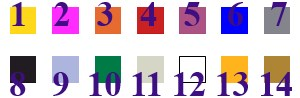
\includegraphics{colors}

\begin{enumerate}
\item 黄 [き] - Yellow
\item ピンク - Pink
\item オレンジ - Orange
\item 赤 [あか] - Red
\item 紫 [むらさき] - Purple
\item 青 [あお] - Blue
\item グレー - Grey
\item 黒 [くろ] - Black
\item シアン - Cyan
\item 緑 [みどり] - Green
\item 銀 [ぎん] - Silver
\item 白 [しろ] - White
\item 金 [きん] - Gold
\item 銅 [どう] - Copper
\end{enumerate}

One thing to note is that many things that should be green in Japanese are actually called blue. For example, a green street light is 青 (blue) even if the physical light is 
green. The same applies to 青芝 [あおしば] (blue lawns) and 青林檎 [あおりんご] (blue apples).

\subsection{Body parts}

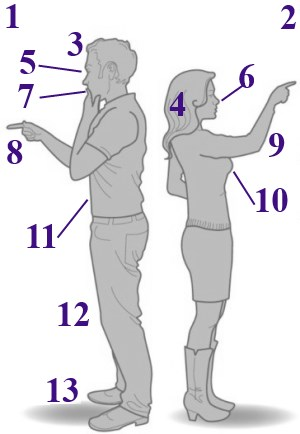
\includegraphics{bodies}

\begin{enumerate}
\item 男 [おとこ], 男の子 - Man, guy
\item 女 [おんな], 女の子 - Woman, girl
\item 頭 [あたま] - Head
\item 髪 [かみ] - Hair
\item 目 [め] - Eyes
\item 鼻 [はな] - Nose
\item 口 [くち] - Mouth
\item 手 [て] - Hand
\item 腕 [うで] - Arm
\item おっぱい - Breasts
\item 腹 [はら] - Belly
\item 脚 [あし], ひざ - Legs, lap
\item 足 [あし] - Feet
\end{enumerate}

\subsection{Requesting help}

Sometimes things go wrong. Here are words related to asking for help, danger and other annoyances:

\begin{colorize}
\item すみません - Excuse me
\item 危ない [あぶない] - Danger
\item 邪魔 [じゃま], めんどくさい - Nuisance
\item 気をつけて [きをつけて] - Be careful
\item ごめんなさい - Sorry
\item ありがとう - Thanks
\item 問題ない [もんだいない] - No problem
\end{colorize}

When requesting something, it's usually best to say \textit{please}. There are two words for it: ください and お願いします [おねがいします]. The first is used when asking for an 
item or an action, while the second is used when requesting a service or wanting to sound more polite. For example: 助けてください [たすけてください] (help please).
\begin{tabular}{@{}|l|l|l|l|@{}}
\hline
\multicolumn{4}{ |c| }{\textbf{助ける [たすける] (to help)}} \\
\hline
I help
&I don't help
&I helped
&Help me!
\\\hline
助ける
&助けない
&助けた
&助けて
\\
助けます
&助けません
&助けました
&
\\ \hline
\end{tabular}

\subsection{Directions}

You can ask where a specific location is in two different ways: 東京はどこですか (Where is Tokyo?) or 東京に行きたいのです (I want to go to Tokyo). Note that any verb can be 
changed into a desire form by adding たい at the end. So 行く (I go) becomes 行きたい (I want to go).

The following are useful to know when trying to find the way somewhere:

\begin{colorize}
\item 右 [みぎ] - Right
\item 左 [ひだり] - Left
\item 真っ直ぐ [まっすぐ] - Straight ahead
\end{colorize}

For example: 駅は左です [えきはひだりです] (the station is to the left).

\clearpage

\section{Education}

This section deals with the concepts of 教育 [きょういく] (education) and 学ぶ [まなぶ] (to study).
\begin{tabular}{@{}|l|l|l|l|@{}}
\hline
\multicolumn{4}{ |c| }{\textbf{学ぶ [まなぶ] (to study)}} \\
\hline
I study
&I don't study
&I studied
&Study!
\\\hline
学ぶ
&学ばない
&学んだ
&学んで
\\
学びます
&学びません
&学びました
&
\\ \hline
\end{tabular}

Here are a few basic school related terms:

\begin{colorize}
\item 学校 [がっこう] - School
\item 高校 [こうこう] - High school
\item 中学校 [ちゅうがっこう] - Middle school
\item 大学校 [だいがっこう] - College
\item 先生 [せんせい] - Teacher
\item 学生 [がくせい] - Student
\item 留学生 [りゅうがくせい] - Foreign exchange student
\item 学校長 [がっこうちょう] - School principal
\item 後輩 [こうはい] - Junior
\item 先輩 [せんぱい] - Senior
\item 試験 [しけん] - Exam
\item 征服 [せいふく] - School uniform
\item 生徒 [せいと] - Student council
\item 生徒会著 [せいとかいちょ] - Student council president
\end{colorize}

Note that 先生 (teacher) can be used for anyone more knowledgeable than you, while 主人 [しゅじん] or マスター (master) is used for people in position of authority. Levels in a 
school are also referred to as 年生 [ねんせい] and used as a counter: 一年生 (first grade), 二年生 (second grade), 三年生 (third grade).

\subsection{Classroom}

Japan schools are all built along very similar plans and concepts. The morning starts with ホームルーム (homeroom) which is when the 先生 (teacher) describes the events of 
the day. Afterward, a 学生 (student) will spend the remainder of the day in the same classroom, except for specialized labs, with teachers swapping rooms.
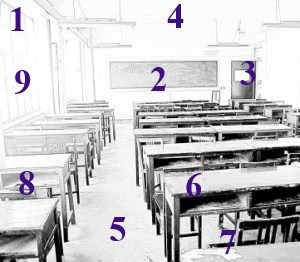
\includegraphics{classroom}

\begin{enumerate}
\item 教室 [きょしつ] - Classroom
\item 黒板 [こくばん] - Blackboard
\item ドア, 障子 [しょうじ] - Door
\item 天井 [てんじょう] - Ceiling
\item 階 [かい] - Floor (counter)
\item 机 [つくえ] - Desk
\item 椅子 [いす] - Chair
\item 教科書 [きょうかしょ] - Textbook
\item 窓 [まど] - Window
\end{enumerate}

Most doors are 障子 (sliding door) as opposed to the western style ドア. Time spent in class typically involve 教科書を分かる [きょうかしょをわかる] (understanding 
the textbook) through repetition and memorization.
\begin{tabular}{@{}|l|l|l|l|@{}}
\hline
\multicolumn{4}{ |c| }{\textbf{分かる [わかる] (to understand)}} \\
\hline
I underst..
&I don't und..
&Understood
&Under..!
\\\hline
分かる
&分からない
&分かった
&分かっ
\\
分かります
&分かりません
&分かりました
&て
\\ \hline
\end{tabular}

The verb 分かる (to understand) can also mean \textit{to know} in certain cases, like when you're expected to know something and you remember it. Otherwise, the verb to use is 知る 
(to know).
\begin{tabular}{@{}|l|l|l|l|@{}}
\hline
\multicolumn{4}{ |c| }{\textbf{知る [しる] (to know)}} \\
\hline
I know
&I don't know
&I knew
&Know!
\\\hline
知る
&知らない
&知った
&知って
\\
知ります
&知りません
&知りました
&
\\ \hline
\end{tabular}

\subsection{Library}

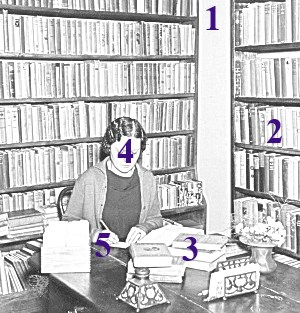
\includegraphics{library}

\begin{enumerate}
\item 図書館 [としょかん] - Library
\item 本棚 [ほんだな] - Bookshelf
\item 本 [ほん] - Book
\item 司書 [ししょ] - Librarian
\item ペン, 鉛筆 [えんぴつ] - Pen, pencil
\end{enumerate}

\subsection{Lunch}

For lunch, most schools in Japan have either the 給食 [きゅうしょく] (school lunch) which is a school provided lunch at a the カフェテリア (cafeteria), or students bring their own 
弁当 [べんとう] (boxed lunch) which they eat in the classroom.

\subsection{Clubs}

After class, most schools have mandatory 部活 [ぶかつ] (club activities). Some popular clubs include 野球 [やきゅう] (baseball), 蹴球 [しゅうきゅう] (soccer), 柔道 [じゅうどう] 
(judo), 剣道 [けんどう] (kendo), テニス (tennis), 水泳 [すいえい] (swimming) and 書道 [しょどう] (calligraphy). These clubs often participate in 文化祭 [ぶんかさい] (culture 
festivals). Some expressions of victory include やった (yay), よかった (that was good) and 了解 [りょうかい] (roger).

\clearpage

\section{Outdoors}

\subsection{Weather}

Telling the 天気 [てんき] (weather) in Japanese is fairly easy. Temperatures are in Celcius and you can describe the overall weather using the following words:

\begin{colorize}
\item 雨 [あめ] - Rain
\item 雪 [ゆき] - Snow
\item 晴 [はれ] - Sunny
\item 雲 [くも] - Cloud
\item 風 [かぜ] - Wind
\item 厚い [あつい] - Hot
\item 寒い [さむい] - Cold
\item 暖かい [あたたかい] - Warm
\item 落雷 [らくらい] - Lightning
\item 台風 [たいふう] - Typhoon
\item 地震 [じしん] - Earthquake
\item 緊急 [きんきゅう] - Emergency
\item 情報 [じょうほう] - Information
\end{colorize}

You can ask for the weather with 今日の天気予報は何ですか [きょうのてんきよほうはなんですか] (What is the weather forecast today?) The answer could be 曇りです (It is cloudy) or 
いい天気になります (The weather will become good).

You can also describe the weather in relation to the various seasons:

\begin{colorize}
\item 春 [はる] - Spring
\item 夏 [なつ] - Summer
\item 秋 [あき] - Autumn
\item 冬 [ふゆ] - Winter
\end{colorize}

\subsection{Animals}

Here are a few common animals you can find outside:

\begin{colorize}
\item 猫 [ねこ], 子猫 [こねこ] - Cat, kitten
\item 犬 [いぬ] - Dog
\item 牛 [うし] - Cow
\item 鴨 [かも] - Duck
\item 熊 [くま] - Bear
\item 兎 [うさぎ] - Rabbit
\end{colorize}

\subsection{Natural landscape}

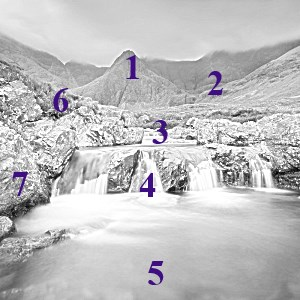
\includegraphics{nature}

\begin{enumerate}
\item 山 [やま] - Mountain
\item 谷 [たに] - Valley
\item 川 [かわ] - River
\item 滝 [たき] - Waterfall
\item 海 [うみ] - Ocean
\item 木 [き] - Tree
\item 岩 [いわ] - Rock
\end{enumerate}

\subsection{City life}

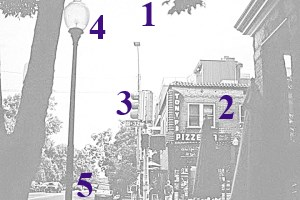
\includegraphics{city}

\begin{enumerate}
\item 市 [いち], 都 [みやこ] - City
\item 棟 [むね] - Building
\item 止まれ [とまれ] - Stop
\item 光 [ひかり] - Light
\item 道 [みち] - Road
\end{enumerate}

Note that the verb 止まる [とまる] (to stop) means to stop as in a vehicle on the street, but 止める [やめる] (to stop) is more commonly used for giving up or resigning.
\begin{tabular}{@{}|l|l|l|l|@{}}
\hline
\multicolumn{4}{ |c| }{\textbf{止める [やめる] (to stop)}} \\
\hline
I stop
&I don't stop
&I stopped
&Stop!
\\\hline
止める
&止めない
&止めた
&止めて
\\
止めます
&止めません
&止めました
&
\\ \hline
\end{tabular}

\subsection{Methods of transport}

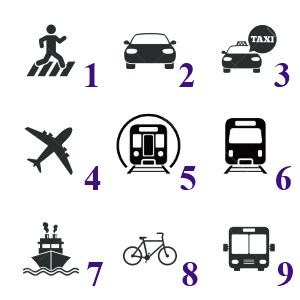
\includegraphics{transport}

\begin{enumerate}
\item 踏み [ふみ] - Steps
\item 車 [くるま] - Car
\item タクシー - Taxi
\item 飛行機 [きこうき] - Airplane
\item 電車 [でんしゃ] - Electric train, subway
\item 列車 [れっしゃ] - Train
\item 船 [ふね] - Boat
\item 自転車 [じてんしゃ] - Bicycle
\item バス - Bus
\end{enumerate}

Japan travel is typically done by train. Other useful train-related terms include 駅 [えき] (train station), 線 [せん] (line) and 切符 [きっぷ], チケット (ticket). To say you will 
walk somewhere, use the verb 歩く [あるく].
\begin{tabular}{@{}|l|l|l|l|@{}}
\hline
\multicolumn{4}{ |c| }{\textbf{歩く [あるく] (to walk)}} \\
\hline
I walk
&I don't walk
&I walked
&Walk!
\\\hline
歩く
&歩かない
&歩いた
&歩いて
\\
歩きます
&歩きません
&歩きました
&
\\ \hline
\end{tabular}

\subsection{At the store}

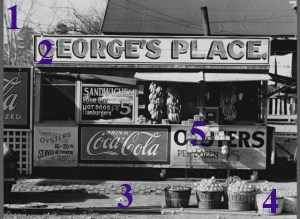
\includegraphics{store}

\begin{enumerate}
\item 店 [みせ] - Store
\item 符号 [ふごう] - Sign
\item 歩道 [ほどう] - Sidewalk
\item 鞄 [かばん] - Bag
\item 棚 [たな] - Shelf
\end{enumerate}

There are many popular stores in Japan including コンビニ (convenience store), コー​​ヒーショップ (coffee shop), 乾物屋 [かんぶつや] (grocery store), 魚屋 [さかなや] (fish market), 
酒屋 [さかや] (liquor store), 本屋 [ほんや] (book store) and スーパー (supermarket).

The act of \textit{shopping} is 買い物する [かいものする], while the verbs are 買う [かう] (to buy) and 売る [うる] (to sell).
\begin{tabular}{@{}|l|l|l|l|@{}}
\hline
\multicolumn{4}{ |c| }{\textbf{買う [かう] (to buy)}} \\
\hline
I buy
&I don't buy
&I bought
&Buy!
\\\hline
買う
&買わない
&買った
&買って
\\
買います
&買いません
&買いました
&
\\ \hline
\end{tabular}
\begin{tabular}{@{}|l|l|l|l|@{}}
\hline
\multicolumn{4}{ |c| }{\textbf{売る [うる] (to sell)}} \\
\hline
I sell
&I don't sell
&I sold
&Sell!
\\\hline
売る
&売らない
&売った
&売って
\\
売ります
&売りません
&売りました
&
\\ \hline
\end{tabular}

\subsection{At the shrine}

Japanese people follow very traditional values. The two main religions are 仏教 [ぶっきょう] (Buddhism) and 神道 [しんとう] (Shinto). Unsurprisingly, 神社 [じんじゃ] (shrines) can be 
found in most locations. These are places of safekeeping for sacred relics and where people pray to 神 [かみ] (God) and wish for good fortune. Many ceremonies are performed at shrines, such as 厄払い [やくばらい] (cleansing of bad luck).
\begin{tabular}{@{}|l|l|l|l|@{}}
\hline
\multicolumn{4}{ |c| }{\textbf{祈る [いのる] (to wish)}} \\
\hline
I wish
&I don't wish
&I wished
&Wish!
\\\hline
祈る
&祈らない
&祈った
&祈って
\\
祈ります
&祈りません
&祈りました
&
\\ \hline
\end{tabular}

Here is some more vocabulary related to traditions and secrets:

\begin{colorize}
\item 秘密 [ひみつ] - Secret
\item 約束 [やくそく] - Promise
\item 化け物 [ばけもの] - Ghost, monster
\end{colorize}

\subsection{At the restaurant}

Meals are typically served as a series of bowls containing various types of food. These are eaten with 端 [はし] (chopsticks) and shared among the people sitting at the table. A 
popular 朝ごはん [あさごはん] (breakfast) meal may look like this:
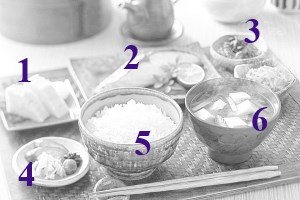
\includegraphics{breakfast}

\begin{enumerate}
\item 卵焼き [たまごやき] - Egg omelette
\item 焼き魚 [やきざかな] - Grilled fish
\item ナット- Fermented soybeans
\item 漬物 [つけもの] - Pickled vegetables
\item ご飯 [ごはん] - Rice
\item 味噌汁 [みそしる] - Miso soup
\end{enumerate}

This can be served with 水 [みず] (water), 酒 [さけ] (liquor) or お茶 [おちゃ] (tea).
\begin{tabular}{@{}|l|l|l|l|@{}}
\hline
\multicolumn{4}{ |c| }{\textbf{飲む [のむ] (to drink)}} \\
\hline
I drink
&I don't drink
&I drank
&Drink!
\\\hline
飲む
&飲まない
&飲んだ
&飲んで
\\
飲みます
&飲みません
&飲みました
&
\\ \hline
\end{tabular}

Some more popular meals, mostly used for snack and 午餐 [ごさん] (dinner), may include:

\begin{colorize}
\item おにぎり - Rice balls
\item すし - Sushi
\item おでん - Oden
\item カレー - Curry
\end{colorize}

\subsection{At the office}

Here are a few common words useful at the office:

\begin{colorize}
\item 会社 [かいしゃ] - Company
\item 会社員 [かいしゃいん] - Office worker
\item 仕事 [しごと] - Work
\item コンピューター - Computer
\item プリンター - Printer
\item メイル - Email
\item 名刺 [めいし] - Business card
\item 電話 [でんわ] - Phone
\item はんこ/印鑑 [はんこいんかん] - Personal stamp
\end{colorize}
\begin{tabular}{@{}|l|l|l|l|@{}}
\hline
\multicolumn{4}{ |c| }{\textbf{働く [はたらく] (to work)}} \\
\hline
I work
&I don't work
&I worked
&Work!
\\\hline
働く
&働かない
&働いた
&働いて
\\
働きます
&働きません
&働きました
&
\\ \hline
\end{tabular}

\clearpage

\section{Inside the home}

A traditional Japanese 家 [いえ] (home) typically starts with a 玄関 [げんかん] (entrance) area where visitors are expected to remove their shoes, followed by one or more rooms for 
daily life. This often includes at least one 畳 [たたみ] (tatami) room, which is a traditional Japanese straw floor covering. The entrance is also where プレゼント (presents) are 
typically given by guests as a sign of appreciation.

\subsection{Living room}

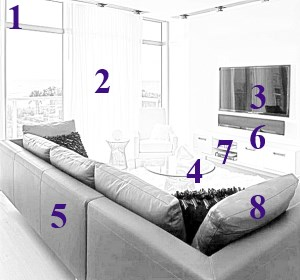
\includegraphics{lr}

\begin{enumerate}
\item リビングルーム - Living room
\item 幔幕 [まんまく] - Curtain
\item テレビ - Television
\item コーヒーテーブル - Coffee table
\item ソファー - Sofa
\item スピーカー - Speakers
\item ゲームコンソール - Games console
\item クッション - Cushion
\end{enumerate}

Some common expressions are modified slightly in Japanese. For example, \textit{turn on the light} is 電気をつけて [でんきをつけて] (use the electricity) while \textit{turn off the 
light} is 電気を消して [でんきをけして] (erase the electricity). Also, the concept of a living room with western style sofas is a new idea. Typically, people would sit on the floor 
around a 炬燵 [コタツ], which would often be the only source of heat in the room.
\begin{tabular}{@{}|l|l|l|l|@{}}
\hline
\multicolumn{4}{ |c| }{\textbf{立つ [たつ] (to stand)}} \\
\hline
I stand
&I don't stand
&I stood
&Stand!
\\\hline
立つ
&立たない
&立った
&立って
\\
立ちます
&立ちません
&立ちました
&
\\ \hline
\end{tabular}
\begin{tabular}{@{}|l|l|l|l|@{}}
\hline
\multicolumn{4}{ |c| }{\textbf{座る [すわる] (to sit)}} \\
\hline
I sit
&I don't sit
&I sat
&Sit!
\\\hline
座る
&座らない
&座った
&座って
\\
座ります
&座りません
&座りました
&
\\ \hline
\end{tabular}

\subsection{Bedroom}

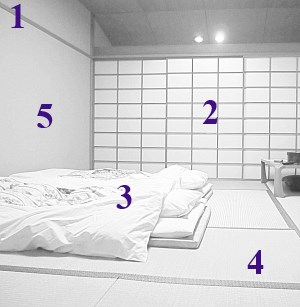
\includegraphics{bedroom}

\begin{enumerate}
\item 寝室 [しんしつ] - Bedroom
\item 障子 [しょうじ] - Sliding door
\item 布団 [ふとん] - Futon
\item 畳 [たたみ] - Tatami carpet
\item 壁 [かべ] - Wall
\end{enumerate}

Most traditional Japanese houses have a 畳 covered floor, however in modern homes this may be found only in the bedroom. Beds are also fairly rare, with people preferring to sleep on 
布団 in the middle of the room, and storing them away in a closet during the day, which gives more space for day time activities.\\
\begin{tabular}{@{}|l|l|l|l|@{}}
\hline
\multicolumn{4}{ |c| }{\textbf{寝る [ねる] (to sleep)}} \\
\hline
I sleep
&I don't sleep
&I slept
&Sleep!
\\\hline
寝る
&寝ない
&寝た
&寝て
\\
寝ます
&寝ません
&寝ました
&
\\ \hline
\end{tabular}
\begin{tabular}{@{}|l|l|l|l|@{}}
\hline
\multicolumn{4}{ |c| }{\textbf{起きる [おきる] (to wake up)}} \\
\hline
I awake
&I don't awake
&I awoke
&Wake up!
\\\hline
起きる
&起きない
&起きた
&起きて
\\
起きます
&起きません
&起きました
&
\\ \hline
\end{tabular}

\subsection{Bathroom}

Most Japanese bathrooms are divided in several rooms for increased convenience. The トイレ (toilet) typically has its own room, then you have a room with one or more シンク (sink), 
and finally a wet room with the シャワー (shower) and 浴 [よく] (bath). The bath water is often reused between family members. Note that bathing is very important to Japanese 
society, and you can find a lot of 銭湯 [せんとう] (public bath) and 温泉 [おんせん] (hot spring) throughout Japan. While many homes have a 洗濯機 [せんたっき] (washing machine), 
most people use a drying line to dry their clothes on the balcony.

\subsection{Kitchen}

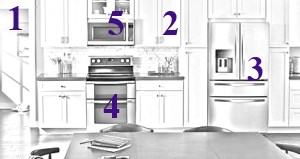
\includegraphics{kitchen}

\begin{enumerate}
\item キッチン - Kitchen
\item 食器棚 [しょっきだな] - Cupboard
\item 冷蔵庫 [れいぞうこ] - Fridge
\item オーブン - Oven
\item 電子レンジ [でんしれんじ] - Microwave
\end{enumerate}
\begin{tabular}{@{}|l|l|l|l|@{}}
\hline
\multicolumn{4}{ |c| }{\textbf{焼く [やく] (to bake, grill)}} \\
\hline
I bake
&I don't bake
&I baked
&Bake!
\\\hline
焼く
&焼かない
&焼いた
&焼いて
\\
焼きます
&焼きません
&焼きました
&
\\ \hline
\end{tabular}

\clearpage

\section{Daily activities}

\subsection{Health}

The most common word related to health is 元気 [げんき] (healthy, energetic) which can be used in the following ways:

\begin{colorize}
\item お元気ですか - How are you?
\item 元気だね - I am well (casual)
\item 元気です - I am well (polite)
\item 元気がない - I am not well (casual)
\item 元気がありません - I am not well (polite)
\end{colorize}

There's no direct way to know whether these sentences refer to someone being sick or simply being out of energy, other than context. To refer specifically to health, use the words 
健康 [けんこう] (health), 健康的 [けんこうてき] (healthy) and 体 [からだ] (body) like this:

\begin{colorize}
\item 健康的人 - This person is healthy
\item ひろしさんは健康的です - Hiroshi is healthy
\item うんどうは健康にいいです - Exercise is good for the health
\item アップルは体にいいです - An apple is good for the body
\item ケーキは体によくない - Cake is not good for the body
\end{colorize}

Other words to describe more serious conditions include 病気 [びょき] (illness), 体調 [たいちょう] (wellness) 病院 [びょういん] (hospital). They can be used like this:

\begin{colorize}
\item 病気です - I'm ill
\item 体調が悪いです - I'm feeling bad
\item 病院にいった - I went to the hospital
\end{colorize}
\begin{tabular}{@{}|l|l|l|l|@{}}
\hline
\multicolumn{4}{ |c| }{\textbf{死ぬ [しぬ] (to die)}} \\
\hline
I die
&I don't die
&I died
&Die!
\\\hline
死ぬ
&死なない
&死んだ
&死んで
\\
死にます
&死にません
&死にました
&
\\ \hline
\end{tabular}

\subsection{Communications}

Most people have a cellphone and can text using SMS, although the most common way to chat is using LINE or Twitter. The easiest way to ask for contact information is with the 
sentence 電話番号教えて [でんわばんごうおしえて] (can you tell me your phone number). To ask someone to repeat, you can use もっとゆっくり話してください (speak more slowly please). 
If you know that you'll be using a specific application such as LINE, you can ask for their 交換 [こうかん] (contact) information with: LINE交換しよう(let's swap LINE contact 
information). To take a break, you can say: やすみましょうか (let's rest)

Here are common sentences used while chatting with friends:

\begin{colorize}
\item おはよう - Morning!
\item 元気? - Are you well?
\item 今日いい天気だね - Nice weather today isn't it?
\item そうだね - Yeah it is.
\item 今何してる? - What are you up to now?
\item テレビ見てる - I'm watching TV
\item ご飯食べてる - I'm eating
\item 今家に帰るところ - I'm about to head home now
\item 今家に出るところ - I'm about to leave home now
\item 映画に行く - I'm going to the cinema
\item 映画に行った - I went to the cinema
\item 今忙しいよ - I'm busy right now
\item 働いてる - I'm working
\item 明日あいてる? - Are you free tomorrow?
\item 明日仕事に行かなきゃ - Tomorrow I have to go to work
\item 土曜日あいてる? - Are you free Saturday?
\item どこ行きたい? - Where do you want to go?
\item コンビニ行かない? - Do you want to go to the convenience store?
\item 笑 / www - lol
\end{colorize}

Note that 行かない (not go) usually implies a negation, however when used in a question it is a way to suggest doing something. It's a softer way to say コンビニ行こ (let's go to 
the convenience store). The same applies for any verb.

Also, adding なきゃ or ないと at the end of a verb implies that you have to do something. For example: 5時までに帰らなきゃ [5じまでにかえらなきゃ] (I have to go home by 5 o'clock) 
or 宿題しなきゃ [しゅくだいしなきゃ] (I have to do homework).

\subsection{Traveling}

Whether this is your first time in Japan or you're trying to navigate some immigration paper work, here are some useful sentences to know when arriving at the airport:

\begin{colorize}
\item パスポートお願いします - Passport, please
\item どうぞ - Here you go
\item ホテルはどこですか - Where is your hotel?
\item しごとですか - Are you here for business?
\item かんこうですか - Are you here for sightseeing?
\end{colorize}

You may also need to know various words that you can find on signs, usually indicating specific locations or actions:

\begin{colorize}
\item 出国審査 [しゅっこくしんさ] - Immigration
\item 税関 [ぜいかん] - Customs
\item 手荷物受取所 [てにもつうけとりじょ] - Baggage claims
\item 第1ターミナル - Terminal 1
\item 出発 [しゅっぱつ] - Departures
\item 到着 [とうちゃく] - Arrivals
\item 乗り継ぎ案内 [のりつぎあんあい] - Connecting flight
\item 出口 [でぐち] - Exit
\item 門口 [かどぐち] - Entrance
\item のぼり - Going up
\item くだり- Going down
\end{colorize}

Once on the ground, it's good to know that Japan is divided into 地方 [ちほう] (regions) such as 関西地方 (Kansai region) and 県, 府 [けん, ふ] (prefectures) such as 東京府 (Tokyo 
prefecture). Train travel is the most common form of transportation on the ground, operated by various regional companies, and large towns are connected by the 新幹線 [しんかんせん] 
(bullet train).

\subsection{Shopping}

Japan is a very cash focused society, so 現金 [げんきん] (cash) is still the standard when going shopping. However, credit cards are becoming more popular, especially in larger 
cities. To find out if the place you're at takes credit cards, you can ask クレジットかアドは使えますか (do you take credit cards). You can also get PASMO cash cards at any 駅 [えき] 
(train station) which can be used to pay for train tickets, subways, but also at some vending machines and stores.

When you're out shopping, you may want to ask これはいくらですか (how much is this) while pointing to an item. For clothes, sizes are referred to as Mサイズ (size medium). So if you 
want a specific item in another size you can say Mサイズがありますか (do you have it in size M). To purchase a specific quantity use the object counter つ like 二つ [ふたつ] (two 
objects). For example, これを二つお願いします (I will take two of these).

Vending machines are also typical of Japan society and contain not only sandwiches and drinks, but also clothing, electronics and hot meals.

Here is a typical dialog between a restaurant owner and client when placing an ご注文 [ごちゅうもん] (order) for 食べ物 [たべもの] (food) and 飲み物 [のみもの] (drinks):

\begin{colorize}
\item いらっしゃいませ - Welcome
\item 何名さまですか - How many people?
\item 二人です - Two people
\item すみません - Excuse me
\item ご注文は - What are you ordering?
\item おすすめ - Your recommendation
\item 見せてあげるは - Let me show you
\item 掛け違えてる [かけちがえてる] - I made a mistake
\item これください - This, please
\item おかわりください - Seconds, please
\item まかせて - Leave it to me
\end{colorize}

\begin{tabular}{@{}|l|l|l|l|@{}}
\hline
\multicolumn{4}{ |c| }{\textbf{あげる (to give)}} \\
\hline
I give
&I don't give
&I gave
&Give!
\\\hline
あげる
&あげない
&あげた
&あげて
\\
あげます
&あげません
&あげました
&
\\ \hline
\end{tabular}

Note that あげる can also be used along with another verb like this: 見せてあげる [みせてあげる] (I will show you) or 教えてあげる [おしえてあげる] (I will teach you).

\subsection{Manga and anime}

While it's hard to classify マンガ (manga) or アニメ (anime) into a specific category, we'll focus more on the "cutesey" type that is typical of this style of entertainment.

Here are some words you can hear in this context:

\begin{colorize}
\item 萌え [もえ] - Precious
\item きゅん - Heart melting
\item 心 [こころ] - Heart
\item 思い出 [おもいで] - Memories
\item 彼女 [かのじょ] - Girlfriend
\item 彼氏 [かれし] - Boyfriend
\item 正義 [せいぎ] - Justice
\item ツンデレ - Tsundere
\item ヤンデレ - Yandere
\item バカ - Idiot
\item 変体 [へんたい] - Perverted
\end{colorize}

A popular saying in a maid caffee would be 萌え, 萌え, きゅん! (moe, moe, kyun!) which basically means something is cute and heart warming. In a more action setting, an anime 
character could say 私は正義です (I am justice).

\subsection{Quantities}

When talking about measurements, Japan uses the same metric system as the rest of the world, so it's easy to translate such numbers. On top of precise quantities, the following words 
can be useful when speaking of one or more objects:

\begin{colorize}
\item すべて - All
\item すべた - Sliced, diced
\item すぎる - Too much
\item 混ぜ [まぜ] - Mixed
\end{colorize}

\subsection{Control panels}

One interesting part of Japanese home life is dealing with control panels to operate common devices such as the bath, shower, toilet and A/C. Most of those use buttons covered by 
kanji. Here are some common symbols found on these controls:

\begin{colorize}
\item 運転 [うんてん] - Turn on/off
\item 切換 [きりかえ] - Switch mode
\item タイマー - Set timer
\item 温く [ぬくく] - Warm water
\item 高温 [こうおん] - Hot water
\item 追炊き [おいだき] - Reheat
\item 冷房 [れいぼう] - Cool air
\item 暖房 [だんぼう] - Hot air
\item 温度 [おんど] - Set temperature
\item おしり - Bidet
\item 大 [だい] - Large amount
\item 小 [こ] - Small amount
\end{colorize}

%\subsection{Technology}

%\subsection{Sciences}


%\subsubsection{Space}

% ehon = picture book
% sasuga = as expected
% moshikashite = by any chance

\end{multicols*}
\end{CJK}
\end{document}

